\chapter{Implementation}
This chapter describes the implementation of GeoDude and some of the considerations as well as the functionality.

\section{GPS module}
The knowledge about pin assignments for the GPS module, RGM-2000, comes from the website: \url{http://www.tobias-schlegel.de/?page_id=51&lang=en}.\\ 
The communication settings were found in the User Manual (RGM-2000\_user\_manual.pdf which can be found in appendix):\\
\begin{table}[H]
    \begin{tabular}{|ll|}
    \hline
    Baud rate    & : 4800 \\ \hline
    Data bit     & : 8    \\ \hline
    Parity       & : None \\ \hline
    Stop bit     & : 1    \\ \hline
    Flow control & : None \\ \hline
    \end{tabular}
\end{table}
To understand the format output from the GPS module, NMEA-0183, we consulted the wikipedia site as well as observing on Tx in RealTerm (terminal software). The raw NMEA-0183 string looks like this:\\
\begin{verbatim}
$GPGGA,092750.000,5321.6802,N,00630.3372,W,1,8,1.03,61.7,M,55.2,M,,*76
\end{verbatim}
To display this data in an understandable way, we have to cut the string up and "send" it. This is done in a smart way in C code:\\
\begin{lstlisting}{language=C}
while((GPSD->gpsstring[j]) != COMMA) // Read lateral string until Comma
{
	GPSD->latString[k] = (GPSD ->gpsstring[j]);
	if(k == 3)
	{
		k++;
		GPSD->latString[k] = '*';   
		// the degree symbol doesnt exist in ascii. 
		// Asterisk is a placeholder
	}
	j++;
	k++;
}
\end{lstlisting}
By running through the GPS string until a comma is found, we can catch every snippet. The snippets are put into string found in the GPSDATA struct. The struct can be found in gps.h (in appendix gps.h.pdf). T

\section{Screen}
The screen is a nokia 3310 display controlled by a PCD8544. The PCD8544 has an SPI interface along with three control pins. These pins are: Chip enable, reset and data/command pin.\\
The data/command pin is used to tell the display whether a command or data has been transmitted. Below a figure from the datasheet is displayed, showing how a transmission should be done.

\begin{figure}[hbpt]
\centering
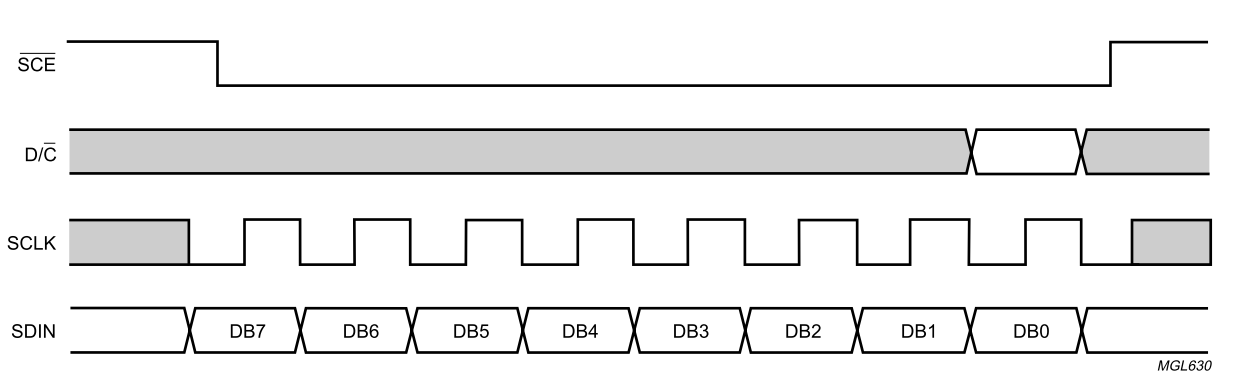
\includegraphics[width=.8\textwidth]{billeder/Display_protocol}
\end{figure}

Commands to the display is used for setup purposes such as contrast, cursor position, ram addressing etc. Data to the display is used to set the pixels to either on or off. The display is divided into "banks" where a bank consists of 8 pixels. It has 6 banks in height and 84 banks in width.\\
Using horizontal addressing of these RAM banks allows for easy writing of chars. Making this neet little trick we can use chars as input to this function and thereby using the function in a similar fasion as "printf".
\begin{lstlisting}{language=C}
void LCD_WriteChar(unsigned char ch)
{
	int i;
	for (i=0; i < ch_width ; i++ )
	{
		LCD_Write_data( pgm_read_byte( &(Font [(ch-32)*5 + i] )));	
	}
	LCD_Write_data(0x00);			
}
\end{lstlisting}
The "Font" array is a large array and are, along with the "Arrow" array (which holds data for the 8 direction arrows), placed in the PROGMEM area. At first it wasn't placed here but when we incorporated FreeRTOS to the project we ran out of space. Placing it in PROGMEM made enough space to support FreeRTOS.\\
Below is shown a little part of the Font array:
\begin{lstlisting}{language=C}
static const unsigned char Font[] PROGMEM =
{
	0x00, 0x00, 0x00, 0x00, 0x00,   // sp 
	0x00, 0x00, 0x2f, 0x00, 0x00,    // ! 
	0x00, 0x07, 0x00, 0x07, 0x00,   // "  
	0x14, 0x7f, 0x14, 0x7f, 0x14,   // #  
	0x24, 0x2a, 0x7f, 0x2a, 0x12,   // $  
	....  
};
\end{lstlisting}

The first spot in the array is the 32nd place in the ascii table, therefore we substract 32 from the ch input in the LCD\_WriteChar function when accessing the array. We also multiply by 5 since each char is 5 pixels wide. We found the Font array via google search.

\section{Magnetometer}
The magnetometer is a HMC6352 and is interfaced using i$^2$c. It is a fully implemented compass with everything handled. It has a register were the setup is written to. We set the magnetometer to 10Hz measurement rate, periodic set/reset on, which is factory default, but we set it to make sure we know how and what it is set to.\\
In the datasheet a table is shown were all responses are described.
\begin{figure}[H]
\centering
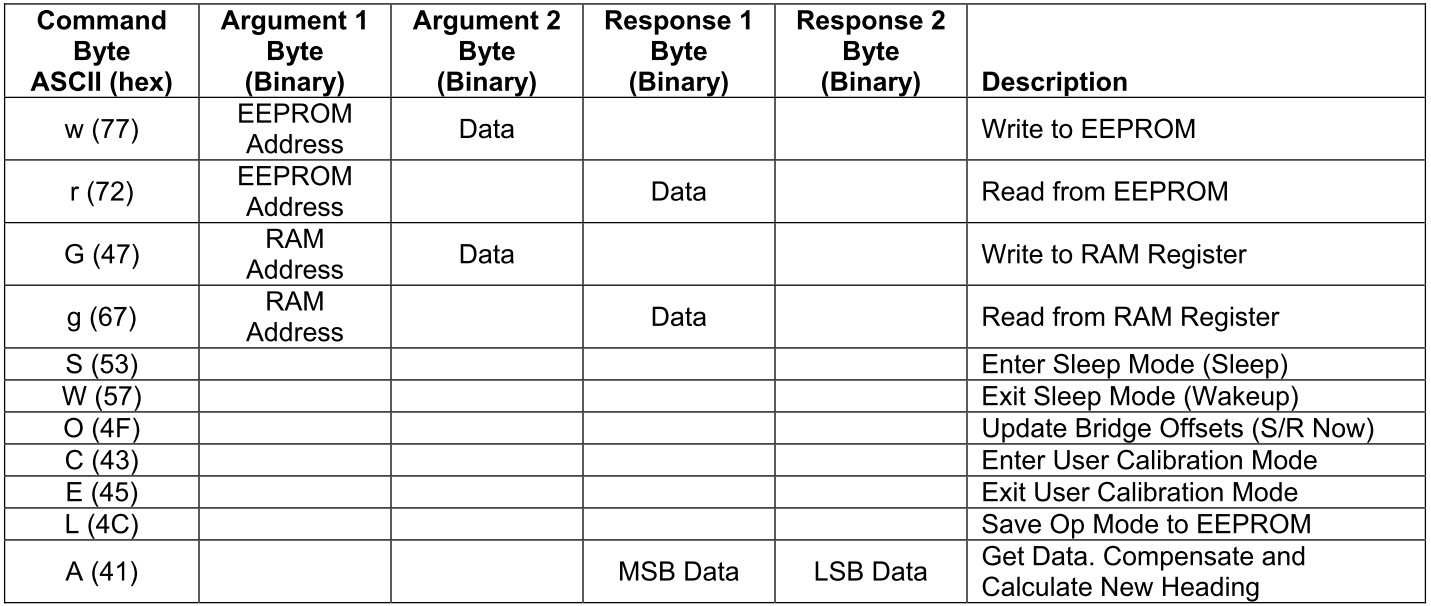
\includegraphics[width=.9\textwidth]{billeder/HMC6352_responses}
\end{figure}
This table was used to identify a transmit/receive sequence. Below is shown an example from the datasheet illustrating a read from a RAM register.
\begin{figure}[H]
\centering
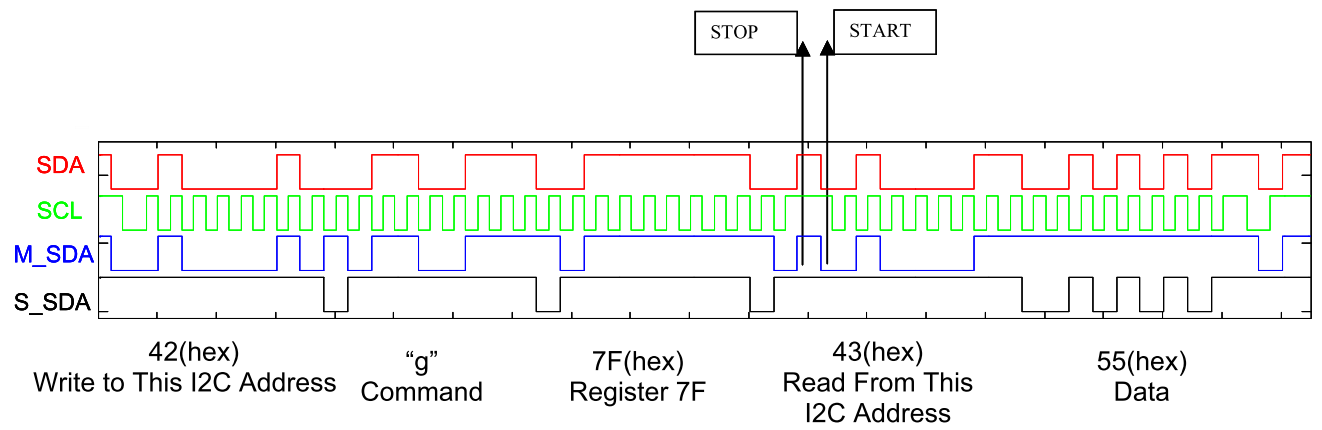
\includegraphics[width=.8\textwidth]{billeder/HMC6352_example}
\end{figure}
A transfer/receive sequence is, as usual in i$^2$c, initated by a "start" from the master by first pulling SDA low and then the SCL. Hereafter the master sends the address indicating a write and then the commands to the slave. When the commands have been sent the transmission is stopped, and then started again shortly after with the read address and the slave responds with the data.\\
There are no pull-up resistors on the HMC6352, these are added externally (see Demo Board).

\section{Software structure}
The software implemented in this project is described by the UML diagram in the figure below.\\
The system is described via. UML even though it is made in C it offers a nice overview of all headers, variables and function calls.
\begin{figure}[hbpt]
\centering
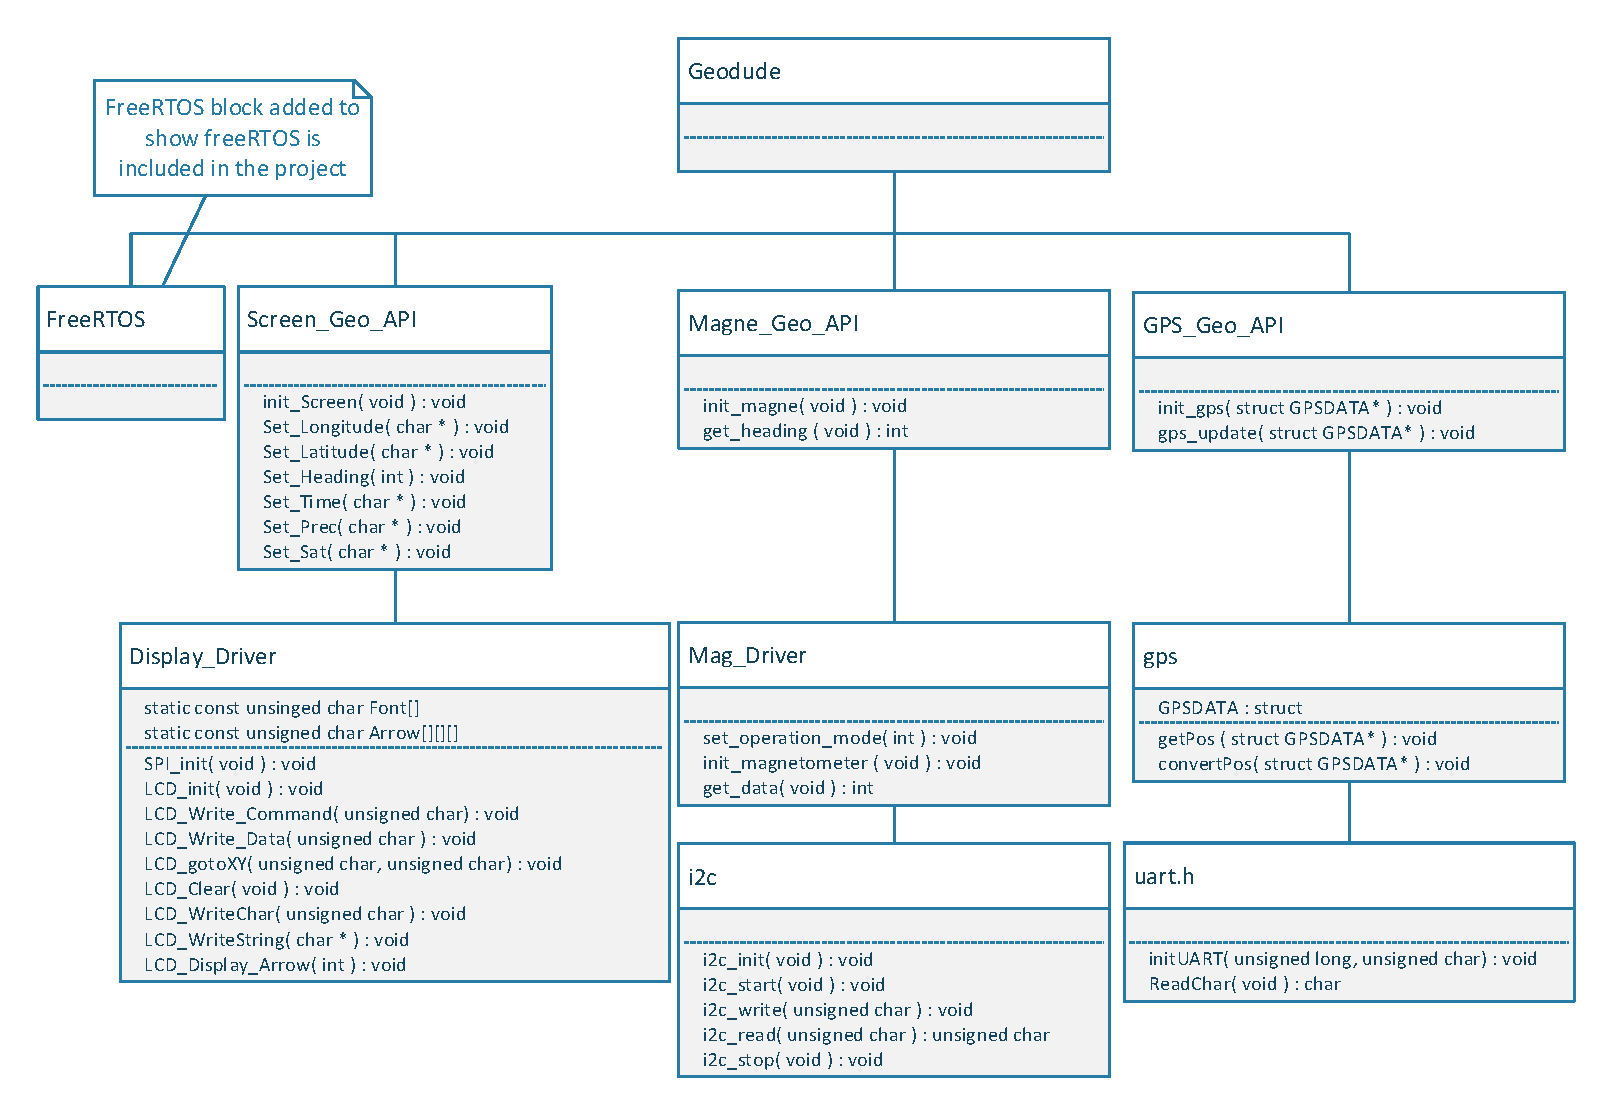
\includegraphics[width=1\textwidth]{billeder/geodude_UML}
\caption{Geodude UML diagram}
\end{figure}

\section{Demo board}
This section briefly describes the demo board developed to make the application portable.

\begin{figure}[H]
\centering
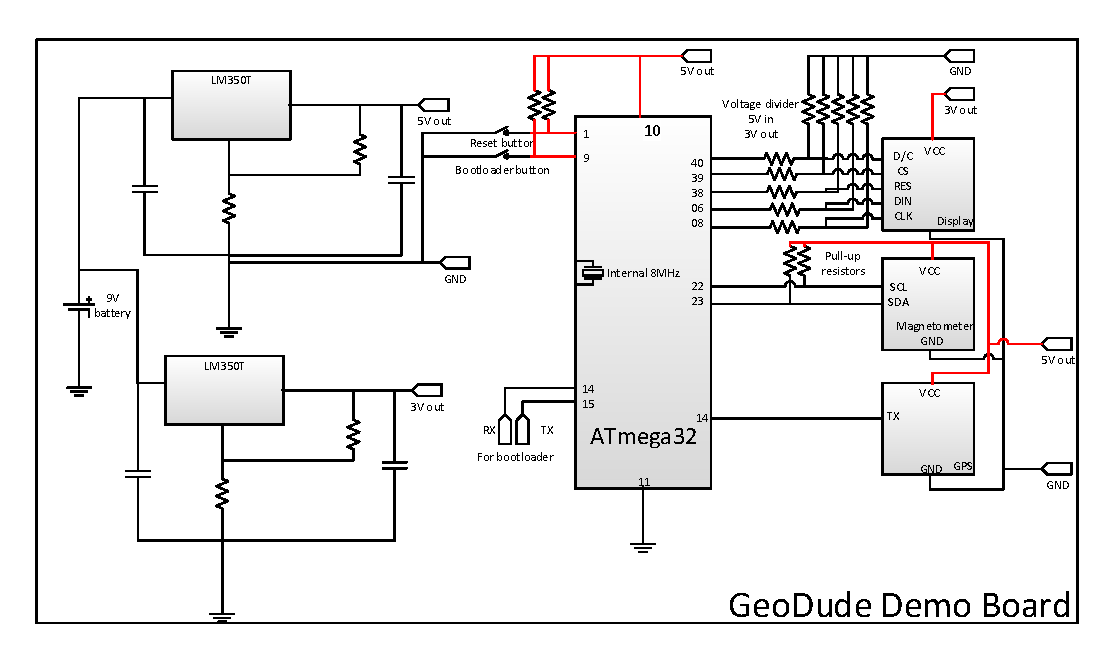
\includegraphics[width=1\textwidth]{billeder/GeodudeDemoBoard}
\end{figure}